\documentclass[14pt]{extarticle}

\begin{document}
	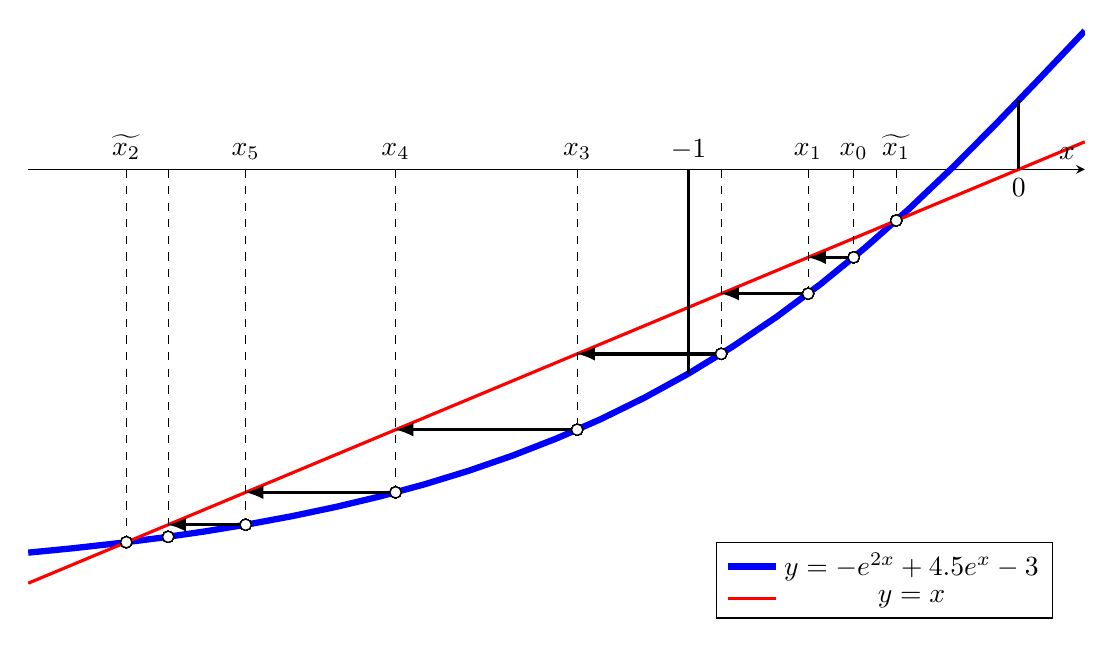
\begin{tikzpicture} [
		declare function= {
			u(\x) = -e^(2*\x) + 4.5 * e^\x - 3;
			i(\x) = \x;
		},]
		\begin{axis} [
			height=10cm,
			width=15cm,
			xlabel = {$x$},
			ylabel = {$y$},
			axis x line = middle,
			hide y axis,
			domain = -3:0.2,
			ticks = none,
			legend pos = south east]

			\newcommand*{\varA}{-1}
			\newcommand*{\varB}{0}
			\newcommand*{\trueXfirst}{-0.371}
			\newcommand*{\trueXsecond}{-2.703}
			\pgfmathsetmacro{\fa}{min(u(\varA), i(\varA))}
			\pgfmathsetmacro{\fb}{max(u(\varB), i(\varB))}
			\pgfmathsetmacro{\Xzeroth}{(\varA+\varB)/2}
			\pgfmathsetmacro{\Xfirst}{u(\Xzeroth)}
			\pgfmathsetmacro{\Xsecond}{u(\Xfirst)}
			\pgfmathsetmacro{\Xthird}{u(\Xsecond)}
			\pgfmathsetmacro{\Xfourth}{u(\Xthird)}
			\pgfmathsetmacro{\Xfifth}{u(\Xfourth)}
			\pgfmathsetmacro{\Xsixth}{u(\Xfifth)}
			\pgfmathsetmacro{\Xseventh}{u(\Xsixth)}
			\pgfmathsetmacro{\Xeighth}{u(\Xseventh)}
			\pgfmathsetmacro{\Xnineth}{u(\Xeighth)}

			\addplot[color=blue, line width=.08cm]{u(x)};
			\addplot[color=red, line width=.04cm]{i(x)};

			\coordinate(A) at 	(\varA,		\fa);
			\coordinate(B) at 	(\varB,		\fb);
			\coordinate(X1true) at 	(\trueXfirst,	\trueXfirst);
			\coordinate(X2true) at 	(\trueXsecond,	\trueXsecond);
			\coordinate(X0) at 	(\Xzeroth,	\Xfirst);
			\coordinate(X1) at 	(\Xfirst,	\Xsecond);
			\coordinate(X2) at 	(\Xsecond,	\Xthird);
			\coordinate(X3) at 	(\Xthird,	\Xfourth);
			\coordinate(X4) at 	(\Xfourth,	\Xfifth);
			\coordinate(X5) at 	(\Xfifth,	\Xsixth);
			\coordinate(X6) at 	(\Xsixth,	\Xseventh);
			\node[above](Ap) at	(\varA,		0) {$\varA$};
			\node[below](Bp) at	(\varB,		0) {$\varB$};
			\node[above](X1trueP)at	(\trueXfirst,	0)
				{$\widetilde{x_1}$};
			\node[above](X2trueP)at	(\trueXsecond,	0)
				{$\widetilde{x_2}$};
			\node[above](X0p) at	(\Xzeroth,	0) {$x_0$};
			\node[above](X1p) at	(\Xfirst,	0) {$x_1$};
			\coordinate(X2p) at	(\Xsecond,	0);
			\node[above](X3p) at	(\Xthird,	0) {$x_3$};
			\node[above](X4p) at	(\Xfourth,	0) {$x_4$};
			\node[above](X5p) at	(\Xfifth,	0) {$x_5$};
			\coordinate(X6p) at	(\Xsixth,	0);
			\coordinate(X0med) at 	(\Xfirst,	\Xfirst);
			\coordinate(X1med) at 	(\Xsecond,	\Xsecond);
			\coordinate(X2med) at 	(\Xthird,	\Xthird);
			\coordinate(X3med) at 	(\Xfourth,	\Xfourth);
			\coordinate(X4med) at 	(\Xfifth,	\Xfifth);
			\coordinate(X5med) at 	(\Xsixth,	\Xsixth);

			\addplot[mark=*,only marks, fill=white]
				(\trueXfirst, \trueXfirst) node[above, pos=1]{};
			\addplot[mark=*,only marks, fill=white]
				(\trueXsecond, \trueXsecond)node[above,pos=1]{};
			\addplot[mark=*,only marks, fill=white]
				(\Xzeroth,\Xfirst) node[above, pos=1]{};
			\addplot[mark=*,only marks, fill=white]
				(\Xfirst,\Xsecond) node[above, pos=1]{};
			\addplot[mark=*,only marks, fill=white]
				(\Xsecond,\Xthird) node[above, pos=1]{};
			\addplot[mark=*,only marks, fill=white]
				(\Xthird,\Xfourth) node[above, pos=1]{};
			\addplot[mark=*,only marks, fill=white]
				(\Xfourth,\Xfifth) node[above, pos=1]{};
			\addplot[mark=*,only marks, fill=white]
				(\Xfifth,\Xsixth) node[above, pos=1]{};
			\addplot[mark=*,only marks, fill=white]
				(\Xsixth,\Xseventh) node[above, pos=1]{};

			\draw[very thick] (Ap) -- (A)		(Bp) -- (B);
			\draw[dashed] (X1trueP) -- (X1true)
				(X2trueP) -- (X2true)	(X0p) -- (X0)
				(X1p) -- (X1)	(X2p) -- (X2)
				(X3p) -- (X3)	(X4p) -- (X4)
				(X5p) -- (X5)	(X6p) -- (X6);

			\draw[-latex, very thick] (X0) edge (X0med) (X1) edge (X1med)
				(X2) edge (X2med) (X3) edge (X3med) (X4) edge (X4med)
				(X5) -- (X5med);

			\addlegendentry{$y=-e^{2x}+4.5e^x-3$};
			\addlegendentry{$y=x$};
		\end{axis}
	\end{tikzpicture}
\end{document}
